\documentclass{article}
\usepackage[spanish]{babel}
\usepackage[a4paper,
            top=2cm,
            bottom=2cm,
            left=3cm,
            right=3cm,
            headheight=36pt,
            nomarginpar,
            includehead,
            includefoot,
            ]{geometry}
\usepackage{graphicx}
\usepackage{listings}
\usepackage{fancyhdr}
\usepackage{parskip}
\usepackage{courier}
\usepackage{xcolor}
\usepackage{minted}


% \usemintedstyle{monokai}
\definecolor{background}{gray}{0.2}


\setminted[python3]{
    style=default,
    % bgcolor=background,
    breaklines,
    linenos=true,
    firstnumber=0,
    fontsize=\footnotesize,
    frame=single,
    samepage=true,
    % xleftmargin=20pt,
    % xrightmargin=20pt,
}


\lstset{
    language=Python,                    % the language of the code
    basicstyle=\footnotesize\ttfamily,  % the size of the fonts that are used for the code
    breakatwhitespace=true,             % sets if automatic breaks should only happen at whitespace
    breaklines=true,                    % sets automatic line breaking
    keepspaces=true,                    % keeps spaces in text, useful for keeping indentation of code (possibly needs columns=flexible)
    escapeinside={\%*}{*)},             % if you want to add LaTeX within your code
    extendedchars=true,                 % lets you use non-ASCII characters; for 8-bits encodings only, does not work with UTF-8
    otherkeywords={None,Entrada,Salida},% if you want to add more keywords to the set
    deletekeywords={del},               % if you want to delete keywords from the given language
    literate=   {á}{{\'a}}1             % fixes utf-8 errors in lstlisting environments
                {é}{{\'e}}1
                {í}{{\'i}}1
                {ó}{{\'o}}1
                {ú}{{\'u}}1,
}


% header & footer settings
\fancyhf{}
\lhead{
\includegraphics[height=32pt]{img/logo-uncuyo-fing.pdf}}
\rhead{ Licenciatura en Ciencias de la Computación \\
        Algoritmos y Estructuras de Datos II \\
        Árboles Balanceados: AVL}
\rfoot{\thepage}
\pagestyle{fancy}


\title{Trabajo Práctico Nº 1}
\author{Gonzalo Padilla}
\date{Marzo 2024}


\begin{document}
\maketitle
\pagestyle{fancy}


\section*{Parte 1}

\textbf{Importante:} Los ejercicios de esta primera parte tienen como objetivo codificar las diferentes funciones básicas necesarias para implementar un árbol AVL.

A partir de estructuras definidas como:

\begin{lstlisting}
class AVLTree:
    root = None

class AVLNode:
    parent = None
    leftnode = None
    rightnode = None
    key = None
    value = None
    bf = None
\end{lstlisting}

Copiar y adaptar todas las operaciones del \textbf{binarytree.py} (i.e. insert(), delete(), search(), etc.) al nuevo módulo \textbf{avltree.py}. Notar que estos luego deberán ser implementados para cumplir que la propiedad de un árbol AVL
\subsubsection*{Solución}
Ver ejercicios 4 y 5.


\subsection*{Ejercicio 1}
Crear un modulo de nombre \textbf{avltree.py}. Implementar las siguientes funciones:
\begin{lstlisting}
%*\textbf{rotateLeft(Tree,avlnode)}*)
    %*\textbf{Descripción}*): Implementa la operación rotación a la izquierda
    Entrada: Un Tree junto a un AVLnode sobre el cual se va a operar la rotación a la izquierda
    Salida: retorna la nueva raíz

%*\textbf{rotateRight(Tree,avlnode)}*)
    %*\textbf{Descripción}*): Implementa la operación rotación a la derecha
    Entrada: Un Tree junto a un AVLnode sobre el cual se va a operar la rotación a la derecha
    Salida: retorna la nueva raíz
\end{lstlisting}
\subsubsection*{Solución}
\inputminted{python3}{./code/snippets/ejercicio1.py}


\subsection*{Ejercicio 2}
Implementar una función recursiva que calcule el elemento balanceFactor de cada subárbol siguiendo la siguiente especificación:
\begin{lstlisting}
%*\textbf{calculateBalance(AVLTree)}*)
    %*\textbf{Descripción}*): Calcula el factor de balanceo de un árbol binario de búsqueda.
    Entrada: El árbol AVL sobre el cual se quiere operar.
    Salida: El árbol AVL con el valor de balanceFactor para cada subarbol
\end{lstlisting}
\subsubsection*{Solución}
\inputminted{python3}{./code/snippets/ejercicio2.py}


\subsection*{Ejercicio 3}
Implementar una funcion en el modulo avltree.py de acuerdo a  las siguientes especifcaciones:

\begin{lstlisting}
%*\textbf{reBalance(AVLTree)}*)
    %*\textbf{Descripción}*): balancea un árbol binario de búsqueda. Para esto se deberá primero calcular el balanceFactor del árbol y luego en función de esto aplicar la estrategia de rotación que corresponda.
    Entrada: El árbol binario de tipo AVL  sobre el cual se quiere operar.
    Salida: Un árbol binario de búsqueda balanceado. Es decir luego de esta operación se cumple que la altura (h) de su subárbol derecho e izquierdo difieren a lo sumo en una unidad.
\end{lstlisting}
\subsubsection*{Solución}
\setlength{\fboxsep}{0pt}
\inputminted{python3}{./code/snippets/ejercicio3.py}


\subsection*{Ejercicio 4}
Implementar la operación \textbf{insert()} en  el módulo \textbf{avltree.py} garantizando que el árbol  binario resultante sea un árbol AVL. 
\subsubsection*{Solución}
\inputminted{python3}{./code/snippets/ejercicio4.py}


\subsection*{Ejercicio 5}
Implementar la operación \textbf{delete()} en  el módulo \textbf{avltree.py} garantizando que el árbol  binario resultante sea un árbol AVL.
\subsubsection*{Solución}
\inputminted{python3}{./code/snippets/ejercicio5.py}


\section*{Parte 2}
\subsection*{Ejercicio 6}
\begin{enumerate}
\item Responder V o F y justificar su respuesta:
\begin{enumerate}
\item \underline{ F } En un AVL el penúltimo nivel tiene que estar completo

El siguiente contra ejemplo demuestra que la proposición es falsa.

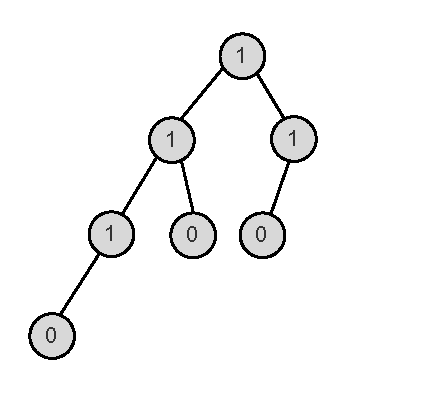
\includegraphics[scale=0.5]{./img/ej6a-arbol.pdf}

Como puede verse, es un AVL ya que el balance factor de cada nodo es -1, 0 o 1, pero su penúltimo nivel está incompleto.

\item \underline{ V } Un AVL donde todos los nodos tengan factor de balance 0 es completo

Un árbol es completo si todos los nodos de todos sus niveles, excepto el último, tienen 2 hijos. Como todos los nodos del árbol tienen balance factor 0, entonces cada uno debe tener 0 hijos, o tener 2 hijos que formen subárboles de la misma altura.

Sea $h$ la altura del árbol, analicemos cada nivel $l$. En el primer nivel $(l=0)$, si $h=l=0$, entonces la raíz deberá tener necesariamente 0 hijos. En tal caso, se tiene un árbol completo, ya que los nodos de su último (y único) nivel tienen 0 hijos. En cambio, si $l\neq h$, entonces necesariamente deberá tener algún hijo. Pero como ya vimos, solo puede tener 0 o 2 hijos, por lo que debe tener 2. Además, los subárboles que formen sus hijos deberán tener ambos la misma altura $h-l-1$.

Ahora analizamos el siguiente nivel $(l=1)$. Se tienen dos posibles casos.
\begin{enumerate}
    \item $(l=h)$ En tal caso, estamos en el último nivel, y por lo tanto cada nodo del mismo debe tener 0 hijos.
    \item $(l<h)$ En este caso, algún nodo debe tener 2 hijos. Pero como dijimos que cada subárbol de este nivel debe tener la misma altura $(h-l)$, entonces \em{todos} los nodos de este nivel tienen 2 hijos. Como cada nodo tiene balance factor 0, entonces sus hijos deben también formar subárboles de la misma altura $h-l-1$.
\end{enumerate}

Y así para cada $l = 1, 2, \dots, h$ Entonces, puede verse que para todos los niveles, excepto el último, cada nodo tiene 2 hijos, entonces se tiene un árbol completo.

\item \underline{ V } En la inserción en un AVL, si al actualizarle el factor de balance al padre del nodo insertado éste no se desbalanceó, entonces no hay que seguir verificando hacia arriba porque no hay cambios en los factores de balance.

Si el balance factor del padre del nodo insertado no se desbalanceó, esto quiere decir que el padre tenía previamente un solo hijo y, por lo tanto, un balance factor de -1 o 1, que pasó luego a 0. Si ya tenía 1 hijo, entonces al agregarle otro a su lado, no cambia la altura del subárbol formado a partir del nodo padre. Por lo tanto, no cambia la altura de ningún subárbol formado a partir de sus nodos superiores, y no es necesario actualizar sus balance factors.

\item \underline{ V } En todo AVL existe al menos un nodo con factor de balance 0.

Todos los nodos terminales tienen balance factor 0, por lo que es verdadero. Si no se toman en cuenta los mismos, entonces la proposición es falsa. Basta tomar un árbol que solo tiene dos nodos: la raíz y un solo hijo. En este caso el hijo es un nodo terminal con balance factor 0, y la raíz, que es el único nodo interior, tiene balance factor 1, entonces el árbol no tiene nodos interior con balance factor 0.

\end{enumerate}
\end{enumerate}


\subsection*{Ejercicio 7}
Sean $A$ y $B$ dos AVL de $m$ y $n$ nodos respectivamente y sea $x$ un key cualquiera de forma tal que para todo key $a\in A$ y para todo key $b\in B$ se cumple que $a < x < b$. Plantear un algoritmo $O(\log n + \log m)$ que devuelva un AVL que contenga los key de $A$, el key $x$ y los key de $B$.
\subsubsection*{Solución}



\subsection*{Ejercicio 8}
Considere una rama truncada en un AVL como un camino simple desde la raíz hacia un nodo que tenga una referencia None (que le falte algún hijo). Demuestre que la mínima longitud (cantidad de aristas) que puede tener una rama truncada en un AVL de altura $h$ es $h/2$ (tomando la parte entera por abajo).

Cualquier camino desde la raíz hasta un nodo que no esté completo puede ser una rama truncada según la definición del ejercicio. Dicho nodo puede no ser necesariamente un nodo hoja.
\subsubsection*{Solución}
Encontrar la longitud mínima que puede tener una rama truncada en un AVL de altura $h$ es equivalente a encontrar la mínima cantidad de niveles completos del mismo. Esto es cierto ya que si el siguiente nivel está completo, entonces todos los nodos del nivel actual tienen 2 hijos (entonces ninguno es el final de una rama truncada), y si el nivel actual no es completo, entonces existe uno con menos de 2 hijos en el nivel anterior (entonces existe una rama truncada de menor longitud al nivel actual).

Podemos encontrar el nivel mínimo completo de un árbol siguiendo los recorridos de menor longitud posible. Si el árbol es de altura $h$, entonces existe un recorrido desde la raíz hasta algún nodo del último nivel, que contiene $h$ aristas y $h+1$ nodos. Para mantener el balance de la raíz, debe existir otro recorrido, que pase por el otro hijo de la raíz, y que tenga altura $h$ o $h-1$. Como nos interesa encontrar el recorrido de menor longitud posible, nos concentramos en el de longitud $h-1$.

De igual forma, desde la perspectiva del hijo de la raíz contenido en este segundo recorrido (en el nivel $n=1$), tal recorrido tiene un altura $h-2$ (comenzando desde el nivel 1), por lo que también debe ser el comienzo de otro recorrido de $h-3$ aristas, que pase por su otro hijo, para mantener su propio balance. En general, en este mínimo recorrido, el nodo del nivel $l$ forma parte de un recorrido que comienza en él, con altura $h-2l$ a partir de si mismo, y debe a su vez ser el comienzo de un recorrido de altura $h-2l-1$.

Nótese que ambos números pueden ser cero o negativos. Cuando el primero sea cero, significa que el nodo de ese nivel es el final del recorrido, y no existe recorrido menor, entonces estamos en el mínimo nivel completo, y el nodo tiene hijos. Intentar armar un recorrido menor a partir de él da una distancia negativa (el segundo número). Si, en cambio, el segundo número es 0, y el primero positivo, quiere decir que para mantener al nodo balanceado, uno de sus hijos puede no existir (pero no ninguno), entonces hemos encontrado también el mínimo nivel completo y, por lo tanto, la longitud mínima de una rama truncada.

Finalmente, tenemos que $h-2l=0$ si $l=\frac{h}{2}$, y que $h-2l-1=0$ si $l=\frac{h-1}{2}$. Si $h$ es par, solo la primera ecuación tiene solución entera, por lo que utilizamos la fórmula correspondiente. De la misma forma, si $h$ es impar, solo la segunda tiene solución entera. La fórmula $l = \lfloor h/2 \rfloor$ logra que alguno de los números sea 0, que es lo que se quería probar.


\section*{Parte 3}
\subsection*{Ejercicios Opcionales}
\begin{enumerate}
    \item Si n es la cantidad de nodos en un árbol AVL, implemente la operación \textbf{height()} en el módulo \textbf{avltree.py} que determine su altura en $O(\log n)$. Justifique el por qué de dicho orden.
    \subsubsection*{Solución}
    \inputminted{python3}{./code/snippets/ejercicioopcional1.py}
    
    \item Considere una modificación en el módulo \textbf{avltree.py} donde a cada nodo se le ha agregado el campo \textbf{count} que almacena el número de nodos que hay en el subárbol en el que él es raíz. Programe un algoritmo $O(\log n)$ que determine la cantidad de nodos en el árbol cuyo valor del key se encuentra en un intervalo $[a, b]$ dado como parámetro. Explique brevemente por qué el algoritmo programado por usted tiene dicho orden.
\end{enumerate}


\end{document}
